\documentclass[english,man]{apa6}

\usepackage{amssymb,amsmath}
\usepackage{ifxetex,ifluatex}
\usepackage{fixltx2e} % provides \textsubscript
\ifnum 0\ifxetex 1\fi\ifluatex 1\fi=0 % if pdftex
  \usepackage[T1]{fontenc}
  \usepackage[utf8]{inputenc}
\else % if luatex or xelatex
  \ifxetex
    \usepackage{mathspec}
    \usepackage{xltxtra,xunicode}
  \else
    \usepackage{fontspec}
  \fi
  \defaultfontfeatures{Mapping=tex-text,Scale=MatchLowercase}
  \newcommand{\euro}{€}
\fi
% use upquote if available, for straight quotes in verbatim environments
\IfFileExists{upquote.sty}{\usepackage{upquote}}{}
% use microtype if available
\IfFileExists{microtype.sty}{\usepackage{microtype}}{}

% Table formatting
\usepackage{longtable, booktabs}
\usepackage{lscape}
% \usepackage[counterclockwise]{rotating}   % Landscape page setup for large tables
\usepackage{multirow}		% Table styling
\usepackage{tabularx}		% Control Column width
\usepackage[flushleft]{threeparttable}	% Allows for three part tables with a specified notes section
\usepackage{threeparttablex}            % Lets threeparttable work with longtable

% Create new environments so endfloat can handle them
% \newenvironment{ltable}
%   {\begin{landscape}\begin{center}\begin{threeparttable}}
%   {\end{threeparttable}\end{center}\end{landscape}}

\newenvironment{lltable}
  {\begin{landscape}\begin{center}\begin{ThreePartTable}}
  {\end{ThreePartTable}\end{center}\end{landscape}}

  \usepackage{ifthen} % Only add declarations when endfloat package is loaded
  \ifthenelse{\equal{\string man}{\string man}}{%
   \DeclareDelayedFloatFlavor{ThreePartTable}{table} % Make endfloat play with longtable
   % \DeclareDelayedFloatFlavor{ltable}{table} % Make endfloat play with lscape
   \DeclareDelayedFloatFlavor{lltable}{table} % Make endfloat play with lscape & longtable
  }{}%



% The following enables adjusting longtable caption width to table width
% Solution found at http://golatex.de/longtable-mit-caption-so-breit-wie-die-tabelle-t15767.html
\makeatletter
\newcommand\LastLTentrywidth{1em}
\newlength\longtablewidth
\setlength{\longtablewidth}{1in}
\newcommand\getlongtablewidth{%
 \begingroup
  \ifcsname LT@\roman{LT@tables}\endcsname
  \global\longtablewidth=0pt
  \renewcommand\LT@entry[2]{\global\advance\longtablewidth by ##2\relax\gdef\LastLTentrywidth{##2}}%
  \@nameuse{LT@\roman{LT@tables}}%
  \fi
\endgroup}


\ifxetex
  \usepackage[setpagesize=false, % page size defined by xetex
              unicode=false, % unicode breaks when used with xetex
              xetex]{hyperref}
\else
  \usepackage[unicode=true]{hyperref}
\fi
\hypersetup{breaklinks=true,
            pdfauthor={},
            pdftitle={Are there strain differences in wheel-running in mice},
            colorlinks=true,
            citecolor=blue,
            urlcolor=blue,
            linkcolor=black,
            pdfborder={0 0 0}}
\urlstyle{same}  % don't use monospace font for urls

\setlength{\parindent}{0pt}
%\setlength{\parskip}{0pt plus 0pt minus 0pt}

\setlength{\emergencystretch}{3em}  % prevent overfull lines

\ifxetex
  \usepackage{polyglossia}
  \setmainlanguage{}
\else
  \usepackage[english]{babel}
\fi

% Manuscript styling
\captionsetup{font=singlespacing,justification=justified}
\usepackage{csquotes}
\usepackage{upgreek}

 % Line numbering
  \usepackage{lineno}
  \linenumbers


\usepackage{tikz} % Variable definition to generate author note

% fix for \tightlist problem in pandoc 1.14
\providecommand{\tightlist}{%
  \setlength{\itemsep}{0pt}\setlength{\parskip}{0pt}}

% Essential manuscript parts
  \title{Are there strain differences in wheel-running in mice}

  \shorttitle{Wheel-running in mice}


  \author{George Washington\textsuperscript{1}~\& Jane Doe\textsuperscript{1,2}}

  \def\affdep{{"", ""}}%
  \def\affcity{{"", ""}}%

  \affiliation{
    \vspace{0.5cm}
          \textsuperscript{1} Jupiter Research University\\
          \textsuperscript{2} Institue of Neuroscience, University of Life  }

 % If no author_note is defined give only author information if available
      \newcounter{author}
                              \authornote{
            Correspondence concerning this article should be addressed to George Washington, 9001 Saturn Lane, Planet Jupiter, 10044. E-mail: \href{mailto:washington@email.com}{\nolinkurl{washington@email.com}}
          }
                                  

  \abstract{In this study we found that strain differences in wheel-running existed
in male mice. We also observed that all strains showed high levels of
wheel running on day 1, the 129S strain showed rapid habituation to
wheel-running and did not continue to run in the wheels to such a high
level by day 4.}
  \keywords{wheel-running, mice, strains, behavior \\

    \indent Word count: X
  }





\usepackage{amsthm}
\newtheorem{theorem}{Theorem}
\newtheorem{lemma}{Lemma}
\theoremstyle{definition}
\newtheorem{definition}{Definition}
\newtheorem{corollary}{Corollary}
\newtheorem{proposition}{Proposition}
\theoremstyle{definition}
\newtheorem{example}{Example}
\theoremstyle{definition}
\newtheorem{exercise}{Exercise}
\theoremstyle{remark}
\newtheorem*{remark}{Remark}
\newtheorem*{solution}{Solution}
\begin{document}

\maketitle

\setcounter{secnumdepth}{0}



\section{Introduction}\label{introduction}

There is a long literature of mice running in wheels (Koteja, Garland,
Sax, Swallow, \& Carter, 1999; Swallow, Carter, \& Garland, 1998). I'm
not going to talk about that here in this introduction. I'm also not
going to talk about the different strains of mice that exist (Beck et
al., 2000; Crawley et al., 1997).

\section{Methods}\label{methods}

We report how we determined our sample size, all data exclusions (if
any), all manipulations, and all measures in the study.

\subsection{Data analysis}\label{data-analysis}

We used R (3.3.0, R Core Team, 2016) and the R-packages \emph{bindrcpp}
(0.2, Muller, 2017), \emph{broom} (0.4.2, Robinson, 2017), \emph{dplyr}
(0.7.4, Wickham, Francois, Henry, \& Muller, 2017), \emph{ggplot2}
(2.2.1, Wickham, 2009), \emph{knitr} (1.17, Xie, 2015), \emph{papaja}
(0.1.0.9492, Aust \& Barth, 2017), \emph{purrr} (0.2.3, Henry \&
Wickham, 2017), \emph{readr} (0.2.2, Wickham \& Francois, 2015),
\emph{tibble} (1.3.4, Muller \& Wickham, 2017), \emph{tidyr} (0.7.1,
Wickham \& Henry, 2017), and \emph{tidyverse} (1.1.1, Wickham, 2017) for
all our analyses.

\newpage

\section{Results}\label{results}

\begin{table}[tbp]
\begin{center}
\begin{threeparttable}
\caption{\label{tab:table1}Summary statistics of wheel running by Strain}
\begin{tabular}{lllll}
\toprule
strain & \multicolumn{1}{c}{Day1 Mean} & \multicolumn{1}{c}{Day2 Mean} & \multicolumn{1}{c}{Day3 Mean} & \multicolumn{1}{c}{Day4 Mean}\\
\midrule
B6 & 8,694.82 & 7,243.21 & 9,857.32 & 11,191.86\\
F1-129B6 & 10,088.11 & 8,394.89 & 9,949.02 & 12,281.45\\
F1-B6129 & 9,115.03 & 9,089.03 & 10,519.40 & 13,445.00\\
S129 & 8,936.41 & 4,611.03 & 3,668.91 & 4,364.08\\
Swiss & 7,148.19 & 8,006.96 & 9,777.04 & 11,641.31\\
\bottomrule
\end{tabular}
\end{threeparttable}
\end{center}
\end{table}

\begin{figure}

{\centering 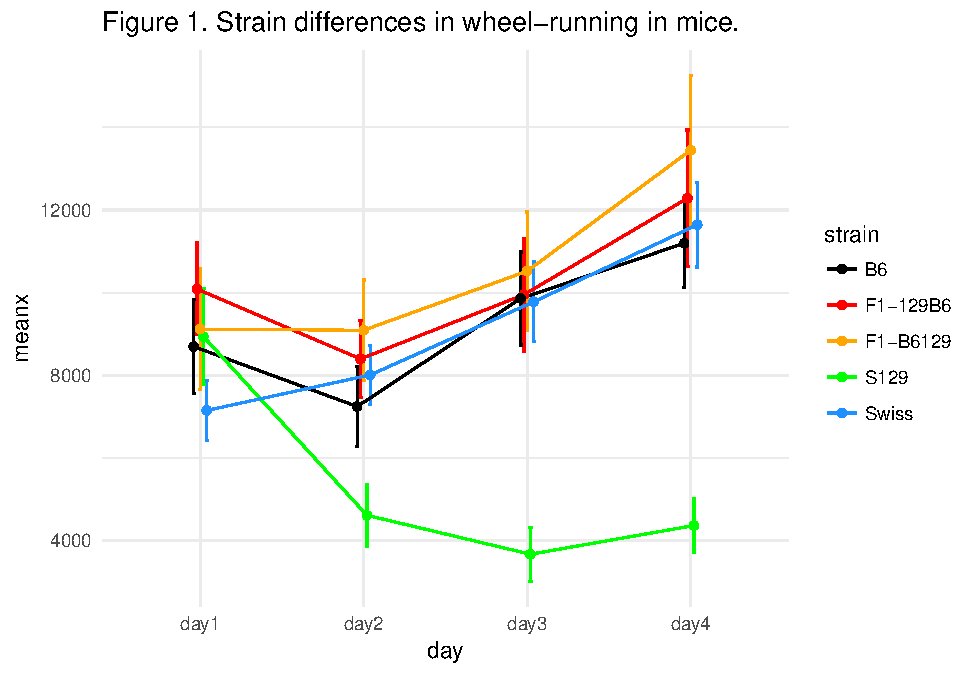
\includegraphics{james_paper_files/figure-latex/fig1-1} 

}

\caption{The S129 strain decreases its wheel-running over successive days.}\label{fig:fig1}
\end{figure}

\begin{table}[tbp]
\begin{center}
\begin{threeparttable}
\caption{\label{tab:table2}Results of Statistical Model}
\begin{tabular}{lllll}
\toprule
term & \multicolumn{1}{c}{estimate} & \multicolumn{1}{c}{std.error} & \multicolumn{1}{c}{statistic} & \multicolumn{1}{c}{p.value}\\
\midrule
(Intercept) & 7,526.78 & 1,031.26 & 7.30 & 0.00\\
strainF1-129B6 & 905.55 & 865.19 & 1.05 & 0.30\\
strainF1-B6129 & 1,281.11 & 927.67 & 1.38 & 0.17\\
strainS129 & -3,749.90 & 946.50 & -3.96 & 0.00\\
strainSwiss & -96.72 & 957.94 & -0.10 & 0.92\\
day & 658.24 & 251.52 & 2.62 & 0.01\\
wheel & 17.97 & 113.44 & 0.16 & 0.87\\
\bottomrule
\end{tabular}
\end{threeparttable}
\end{center}
\end{table}

\begin{figure}

{\centering 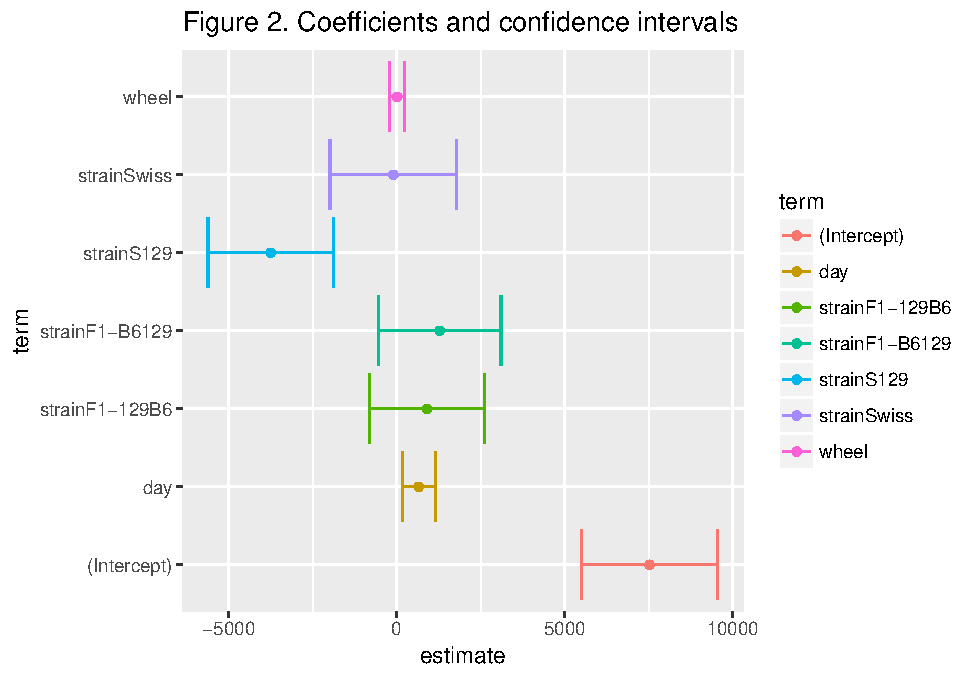
\includegraphics{james_paper_files/figure-latex/fig2-1} 

}

\caption{Output of statistical model}\label{fig:fig2}
\end{figure}

We found that all mice ran in the wheels to a high level (Table
1)\ref{tab:table1}. The most revolutions run by any mouse on any day was
30,463.50. Four out of five strains increased their wheel-running for
each of the successive three days. However, S129 mice decreased their
wheel running over successive days (Figure 1) \ref{fig:fig1}.

Although there was a clear effect of strain and day on wheel-running, we
did not find any evidence that the wheel used was associated with
differences in the number of revolutions made (Figure 2 \ref{fig:fig2}
\& Table 2 \ref{tab:table2} ).

\section{Discussion}\label{discussion}

I have said nearly everything I have to say about this study\footnote{If
  you're still intrigued by wheel-running more info is here:
  \url{http://www.sciencedirect.com/science/article/pii/S0003347299912708}.}.
I do have one more thing to add though.\footnote{Actually I don't.}

\section{Author contributions}\label{author-contributions}

GW and JD designed the experiment and undertook data analysis. GW
performed the experiments. JD drafted the manuscript. GW and JD wrote
and approved the final version of the manuscript for submission.

\section{Acknowledgments}\label{acknowledgments}

We thank all scientists.

\newpage

\section{References}\label{references}

\setlength{\parindent}{-0.5in} \setlength{\leftskip}{0.5in}

\hypertarget{refs}{}
\hypertarget{ref-R-papaja}{}
Aust, F., \& Barth, M. (2017). \emph{papaja: Create APA manuscripts with
R Markdown}. Retrieved from \url{https://github.com/crsh/papaja}

\hypertarget{ref-beck2000genealogies}{}
Beck, J. A., Lloyd, S., Hafezparast, M., Lennon-Pierce, M., Eppig, J.
T., Festing, M. F., \& Fisher, E. M. (2000). Genealogies of mouse inbred
strains. \emph{Nature Genetics}, \emph{24}(1), 23--25.

\hypertarget{ref-crawley1997behavioral}{}
Crawley, J. N., Belknap, J. K., Collins, A., Crabbe, J. C., Frankel, W.,
Henderson, N., \ldots{} others. (1997). Behavioral phenotypes of inbred
mouse strains: Implications and recommendations for molecular studies.
\emph{Psychopharmacology}, \emph{132}(2), 107--124.

\hypertarget{ref-R-purrr}{}
Henry, L., \& Wickham, H. (2017). \emph{Purrr: Functional programming
tools}. Retrieved from \url{https://CRAN.R-project.org/package=purrr}

\hypertarget{ref-koteja1999behaviour}{}
Koteja, P., Garland, T., Sax, J. K., Swallow, J. G., \& Carter, P. A.
(1999). Behaviour of house mice artificially selected for high levels of
voluntary wheel running. \emph{Animal Behaviour}, \emph{58}(6),
1307--1318.

\hypertarget{ref-R-bindrcpp}{}
Muller, K. (2017). \emph{Bindrcpp: An 'rcpp' interface to active
bindings}. Retrieved from
\url{https://CRAN.R-project.org/package=bindrcpp}

\hypertarget{ref-R-tibble}{}
Muller, K., \& Wickham, H. (2017). \emph{Tibble: Simple data frames}.
Retrieved from \url{https://CRAN.R-project.org/package=tibble}

\hypertarget{ref-R-base}{}
R Core Team. (2016). \emph{R: A language and environment for statistical
computing}. Vienna, Austria: R Foundation for Statistical Computing.
Retrieved from \url{https://www.R-project.org/}

\hypertarget{ref-R-broom}{}
Robinson, D. (2017). \emph{Broom: Convert statistical analysis objects
into tidy data frames}. Retrieved from
\url{https://CRAN.R-project.org/package=broom}

\hypertarget{ref-swallow1998artificial}{}
Swallow, J. G., Carter, P. A., \& Garland, T. (1998). Artificial
selection for increased wheel-running behavior in house mice.
\emph{Behavior Genetics}, \emph{28}(3), 227--237.

\hypertarget{ref-R-ggplot2}{}
Wickham, H. (2009). \emph{Ggplot2: Elegant graphics for data analysis}.
Springer-Verlag New York. Retrieved from \url{http://ggplot2.org}

\hypertarget{ref-R-tidyverse}{}
Wickham, H. (2017). \emph{Tidyverse: Easily install and load 'tidyverse'
packages}. Retrieved from
\url{https://CRAN.R-project.org/package=tidyverse}

\hypertarget{ref-R-readr}{}
Wickham, H., \& Francois, R. (2015). \emph{Readr: Read tabular data}.
Retrieved from \url{https://CRAN.R-project.org/package=readr}

\hypertarget{ref-R-tidyr}{}
Wickham, H., \& Henry, L. (2017). \emph{Tidyr: Easily tidy data with
'spread()' and 'gather()' functions}. Retrieved from
\url{https://CRAN.R-project.org/package=tidyr}

\hypertarget{ref-R-dplyr}{}
Wickham, H., Francois, R., Henry, L., \& Muller, K. (2017). \emph{Dplyr:
A grammar of data manipulation}. Retrieved from
\url{https://CRAN.R-project.org/package=dplyr}

\hypertarget{ref-R-knitr}{}
Xie, Y. (2015). \emph{Dynamic documents with R and knitr} (2nd ed.).
Boca Raton, Florida: Chapman; Hall/CRC. Retrieved from
\url{https://yihui.name/knitr/}






\end{document}
